%%%%%%%%%%%%%%%%%%%%%%%%%%%%%%%%%%%%%%%%%
% Simple Sectioned Essay Template
% LaTeX Template
%
% This template has been downloaded from:
% http://www.latextemplates.com
%
% Note:
% The \lipsum[#] commands throughout this template generate dummy text
% to fill the template out. These commands should all be removed when 
% writing essay content.
%
%%%%%%%%%%%%%%%%%%%%%%%%%%%%%%%%%%%%%%%%%

%----------------------------------------------------------------------------------------
%	PACKAGES AND OTHER DOCUMENT CONFIGURATIONS
%----------------------------------------------------------------------------------------

\documentclass[12pt]{article} % Default font size is 12pt, it can be changed here

\usepackage{synttree}
\usepackage{longtable}
\usepackage{geometry} % Required to change the page size to A4

\geometry{a4paper} % Set the page size to be A4 as opposed to the default US Letter

\usepackage{graphicx} % Required for including pictures

\usepackage{float} % Allows putting an [H] in \begin{figure} to specify the exact location of the figure
\usepackage{wrapfig} % Allows in-line images such as the example fish picture

\usepackage{lipsum} % Used for inserting dummy 'Lorem ipsum' text into the template

\linespread{1.2} % Line spacing

%\setlength\parindent{0pt} % Uncomment to remove all indentation from paragraphs

\graphicspath{{./Pictures/}} % Specifies the directory where pictures are stored

\begin{document}

%----------------------------------------------------------------------------------------
%	TITLE PAGE
%----------------------------------------------------------------------------------------

\begin{titlepage}

\newcommand{\HRule}{\rule{\linewidth}{0.5mm}} % Defines a new command for the horizontal lines, change thickness here

\center % Center everything on the page

\textsc{\LARGE University of Glasgow}\\[1.5cm] % Name of your university/college
\textsc{\Large Safety Critical Systems 4}\\[0.5cm] % Major heading such as course name

\HRule \\[0.4cm]
{ \huge \bfseries Safety Analysis Tool\\ for a Foruma 1 Race }\\[0.4cm] % Title of your document
\HRule \\[1.5cm]

\begin{minipage}{0.4\textwidth}
\begin{flushleft} \large
\emph{Author:}\\
Garry \textsc{Sharp}\\ % Your name
\textsc{0801585s}
\end{flushleft}
\end{minipage}
~
\begin{minipage}{0.4\textwidth}
\begin{flushright} \large
\emph{Course Co-Ordinator:} \\
Dr. Chris \textsc{Johnson} % Supervisor's Name
\end{flushright}
\end{minipage}\\[4cm]

{\large 19th of November 2012}\\[3cm] % Date, change the \today to a set date if you want to be precise

%\includegraphics{Logo}\\[1cm] % Include a department/university logo - this will require the graphicx package

\vfill % Fill the rest of the page with whitespace

\end{titlepage}

%---
% Prelude
%----

\begin{abstract}

Formula 1 has always been a sport in which tragedy has had the misfortune to echo throughout its history. The often fervent debate surrounding the sport's safety has lead to much increased safety standards within the past 30 years as there has not been a death in the sport for many years now (although there have been recent deaths in similar sports MotoGP and Indy 500). However, the sport transitioning into a new era has brought about new threats and concerns to both drivers and members of the public. A good example of this could be the terrorist threats this year in advance of the Bahrain GP.

After the infamous death of Aryton Senna in Imola on the 1st of May 1994 (and Roland Ratzenberger in qualifying the day before), many pioneered for increased standards within the sport. Although the actual rate of innovation in safety after this did not increase at all. Innovations continued to be made before the deaths of Senna and Ratzenberger (such as mandatory fire proof clothing for all pit crew and the introduction of a safety car after crashes). The generally acc

This tool aims to objectively quantify the risks involved at any specific race by accepting an array of conditions as an input and then contrasting the likelihood of these conditions to occur and cause an accident with that of the presumed and generally accepted effectiveness of the measures designed to counteract them. The focal point of safety will be on that of the drivers, although, there will invariably be some cross over with other people included in a formula 1 event, this will be especially highlighted when this impacts on the driver in some way.

\end{abstract}

\newpage

%----------------------------------------------------------------------------------------
%	TABLE OF CONTENTS
%----------------------------------------------------------------------------------------

\tableofcontents % Include a table of contents

\newpage % Begins the essay on a new page instead of on the same page as the table of contents 

%----------------------------------------------------------------------------------------
%	Safety in Foruma 1
%----------------------------------------------------------------------------------------

\section{Introduction to Safety in Formula 1} % Major section

We will examine what has happened in previous Foruma 1 events, the consequences of some of these events as well as
continuing innovations in safety in the sport. The governing body of Formula 1 is the FIA (Federation Internationale de l'Automobile), who are a very well known name in Formula 1 and all motorsport throughout the world. The responsibility of the safety of the drivers and other members of the Formula 1 team is their responsibility. Nowadays, and all of their regulations for the current season can be found on their website {\bf FIA reference}.\\
Example citation \cite{Figueredo:2009dg}.\\

%------------------------------------------------

\subsection{Summary of Previous Disaters} % Sub-section

\lipsum[1] % Dummy text

%------------------------------------------------

\subsection{Preventative Measures Taken} % Sub-section
\subsubsection{In General}
\lipsum[2] % Dummy text
\subsubsection{For the 2012 Season}
\lipsum[3] % Dummy text

\begin{figure}[H] % Example image
\center{
\includegraphics[width=0.5\linewidth]{placeholder}}
\caption{Example image.}
\label{fig:speciation}
\end{figure}

%------------------------------------------------

\subsubsection{Subsubsection 2} % Sub-sub-section

\lipsum[4] % Dummy text

\synttree[A[B][C]]

%----------------------------------------------------------------------------------------
%	MAJOR SECTION 1
%----------------------------------------------------------------------------------------

\section{Safety Analysis} % Major section

Any seasoned formula 1 fan will tell you that no two races are ever the same, this of course is true for many sporting event, however, where formula 1 (and motorsport in general) differ is that each driver is in command of a machine that can cause immense damage to other drivers.

%------------------------------------------------

\subsection{Tool Description}

I've elected to use the FMECA technique in the development of the tool, the tool will examine a series of failure modes and after entering certain values, output to a risk matrix the Risk Probablility Number. The values required to calculate the RPN (The severity, occurance and detection rates) will be acquired by calculating user input. There will also be a slight amount of cross over between failure modes (for instance if one of the Electronica Control Units or ECUs breaks in a formula 1 car, then the chances of being forewarned of catastrophic engine failure is drastically reduced), for this reason an overall rating will be given which better reflects the probablilty of an overall accident. The tool also features an ability to view all of the FIA regulations relating to a microcosm of foruma 1 safety, such a pit lane regulations.

\subsection{Block Diagrams}

Placeholder for block diagrams

\subsection{Failure modes}

Place table here

\subsection{Unpredicable Events \& Human Factors} % Sub-section


\begin{wrapfigure}{l}{0.50\textwidth} % Inline image example
  \begin{center}
    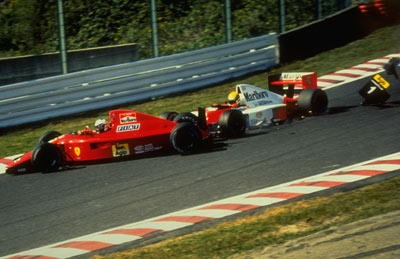
\includegraphics[width=0.45\textwidth]{senna-prost}
  \end{center}
\parbox{7cm}{\caption{Aryton Senna deliberately runs Alain Prost off the track at Suzuka in the 1990 Japan Grand Prix}}
\end{wrapfigure}

It is not always the case in Formula 1 events that the drivers necessarily reflect the risks involved in their racing style. Even after performing a throurough FMECA risk assessment, should a driver or a member of the public exercise a pre-mediated stunt (or simply do something entirely stupid) then there are only certain provisions that can be put in place to handle the resulting events. Figure 2 famously shows Aryton Senna crashing into Alain Prost after feeling cheated that he did not start on the correct side of the track. Although neither driver was injured and safety provisions had been put in place, other than the FIA changing the grid block positions, their is not a lot that they could have done to have prevented the crash. This level of recklessness is not uncommon in formula 1. Indeed a false start by Romain Grojean at Spa this season created a similar crash where he instantly caused three cars (including his own) to be retired straight away. The FIA punished him accordingly and he received a race ban. 

Failure Modes:

\begin{center}
	\begin{longtable}{p{4cm} | p{6cm}| p{6cm}}
		Failure Mode & Local Effect/s & Overall Effect/s \\
		\hline \hline
		Unpredicatable mechanical failure resulting in halting of vehicle & 
			\begin{description} \item{Causes vehicle to veer off track} \item{Whiplash is caused to the driver} \item{Crash with other nearby drivers}
			\end{description} & 
			\begin{description} \item{Fill in} \item{Fill in} \item{Fill in}
			\end{description}\\ \hline


		Unpredicatable mechanical failure without vehicle stop &
			\begin{description} \item{Fill in} \item{Fill in} \item{Fill in}
			\end{description} & 
			\begin{description} \item{Fill in} \item{Fill in} \item{Fill in}
			\end{description}\\ \hline

		Incorrect tyre fitting in pit lane &
			\begin{description} \item{Tyre come loose, reducing steering} \item{Tyre comes off completely}
			\end{description} & 
			\begin{description} \item{Reduced steering results in a bad manouever by the driver, causing either a crash or the driver the beach the car} \item{Car retires in the outer pit lane, obstructing traffic}
			\end{description}\\ \hline


		Speeding in pit lane & %This could enhance the effect of a crash as a result of an incorrect tyre fitting
			\begin{description} \item{Less time to react to sudden activity change in the outer pit lane} \item{Harder to judge entry speed into inner pit lane}
			\end{description} & 
			\begin{description} \item{Increased liklihood of a crash (especially in the event of the above failure mode)}
			\end{description}\\ \hline


		Spectator movement outside of permitted area &
			\begin{description} \item{Less time to react to sudden activity change in the outer pit lane} \item{Harder to judge entry speed into inner pit lane}
			\end{description} & 
			\begin{description} \item{Increased liklihood of a crash (especially in the event of the above failure mode)}
			\end{description}\\ \hline


		Statistical feedback (ECT) broken &
			\begin{description} \item{Little or no meanful feedback from car to team}
			\end{description} & 
			\begin{description} \item{Much harder to predict engine failure, tyre failure or any other mechanical failure, resulting in a decreased detection factor for failure modes based on physical attributes of the car}
			\end{description}\\ \hline


		Team radio broken &
			\begin{description} \item{Little or no meaningful information exchanged between the driver and team}
			\end{description} & 
			\begin{description} \item{Drivers ability to handle an event (such as avoiding debris further down the track) is reduced due to lack of communication}
			\end{description}\\ \hline


		Poorly executed overtaking manouever \\ \hline


		Punctured tyre \\ \hline


		Safety car mechanical failure \\ \hline


		Minor driver fatigue \\ \hline


		Major driver fatigue \\ \hline


		False start \\ \hline
		
	\end{longtable}
\end{center}

%------------------------------------------------

%------------------------------------------------

\subsection{Subsubsection 3} % Sub-sub-section

\begin{description} % Numbered list example

\item[First] \hfill \\
\lipsum[9] % Dummy text

\item[Second] \hfill \\
\lipsum[10] % Dummy text

\item[Third] \hfill \\
\lipsum[11] % Dummy text

\end{description} 

%----------------------------------------------------------------------------------------
%	EVALUATION
%----------------------------------------------------------------------------------------

\subsection{Evaluation}

Due to the scale and nature of Formula 1 events, it would be extremely difficult to do any practical testing of the system. That does not, however, not mean that general testing regarding the method and techniques cannot be performed. A reasonable way of going about the evaluation of the system would be to compare and contrast it to existing systems, and by careful examination of results, make a conculsion based on the accuracy of the system. It should be noted that initial sanity testing against a similar system resulted in a significant change of code, meaning that the version submitted is actually version 3 (with two major re-writes prior to this version), this means that some of the points made in this system have already been changed and will not be visible for 

\subsubsection{Significant Changes to the System}

After the initial implementation (along with basic sanity testing and comparison to a peer's model) it became apparent that a few things needed to be drastically changed, some of these changes can be documented below
\begin{center}
\begin{tabular}{p{3cm} p{10cm}}
Previous Item & Revision \\
\hline \\
Interface \& Interactivity & My initial system had been entirely paper based, it basically operated in a traditional paper based FMECA manner (a simple worksheet). I very quickly realised that making the system more interactive would allow for better, more personalised feedback to be given. I therefore started on a simple HTML mockup of the worksheet. This later changed again to be reflected in a risk matrix. \\
Criticality Analysis & The initial system also did not feature any criticality analysis (this was mostly so that I could see what a more basic mock up of the system would look like before adding functionality), the addition of the criticality analysis feature was not something that I considered would pose that much more of a problem given the scope that I was working in, this was the major inspiration behind the development of the risk matrix. \\
\end{tabular}
\end{center}

\subsubsection{Effectiveness of the Tool}

The tool in general seems to function as desired (basic black box testing showed that it output the correct values when given an input certain input set). What still remains unclear is how well the system would function should it be employed in the safety critical analysis of a Foruma 1 event. As this system focusses on the broader idea of Fromula 1 driver safety and not a particular aspect of it, it has been very difficult to go into detail that, in a real race, would be sufficient enough to perform a serious and accurate test. The current list of FIA regulations spans many many pages, with each racing team adhering to these instructions as well as taking their own safety precautions. Although my tool addresses a subset of each of the safety aspects of a formula 1 race (spectator positioning, pit lane procedures, racing manouevers etc), it does not go as deep as to asses the criticality of each FIA regulation, and as such, cannot possibly claim to be more substantial than the already existing system. That said, in terms of providing a summary (which could be used when presenting a general and overall danger at an event) I would claim that my tool is quite effective. I think its greatest strength is when used in conjuntion with another tool or the general regulatory FIA risk assessment, but not as the primary tool in safety analysis.

Another factor to consider is that lots of the numbers used to generate the RPNs are constructed using inituition and research where available. For instance, it would be very logical to presume that the detecability of a brake failure would be more likely should the brakes be checked before the race. However, as a system which attempts to output quantitative data, it is very difficult to say indefinitely that this increases the detectability by a factor of x. As a fan of Formula 1 I have used values (where applicable) that I believe to be close to what the actual values would be. This means that any RPN that is output to the risk matrix is not entirely accurate, rather, an approximation of the liklihood of an event against its detectability.


%Highlight that it would never realistically get used. FIA are a v.large and responsible organisation. Safety in F1 has already increased significantly

%----------------------------------------------------------------------------------------
%	Findings & Conclusions
%----------------------------------------------------------------------------------------

\section{Findings & Conclusions}
\subsection{Further Development}
In my opinion, there are two ways in which the system can be made to be more accurate
\subsection{Conclusive Summary}

%----------------------------------------------------------------------------------------
%	BIBLIOGRAPHY
%----------------------------------------------------------------------------------------

\begin{thebibliography}{99} % Bibliography - this is intentionally simple in this template

\bibitem[Figueredo and Wolf, 2009]{Figueredo:2009dg}
Figueredo, A.~J. and Wolf, P. S.~A. (2009).
\newblock Assortative pairing and life history strategy - a cross-cultural
  study.
\newblock {\em Human Nature}, 20:317--330.
 
\end{thebibliography}

%----------------------------------------------------------------------------------------

\end{document}